\begin{figure}[t]
    \centering
    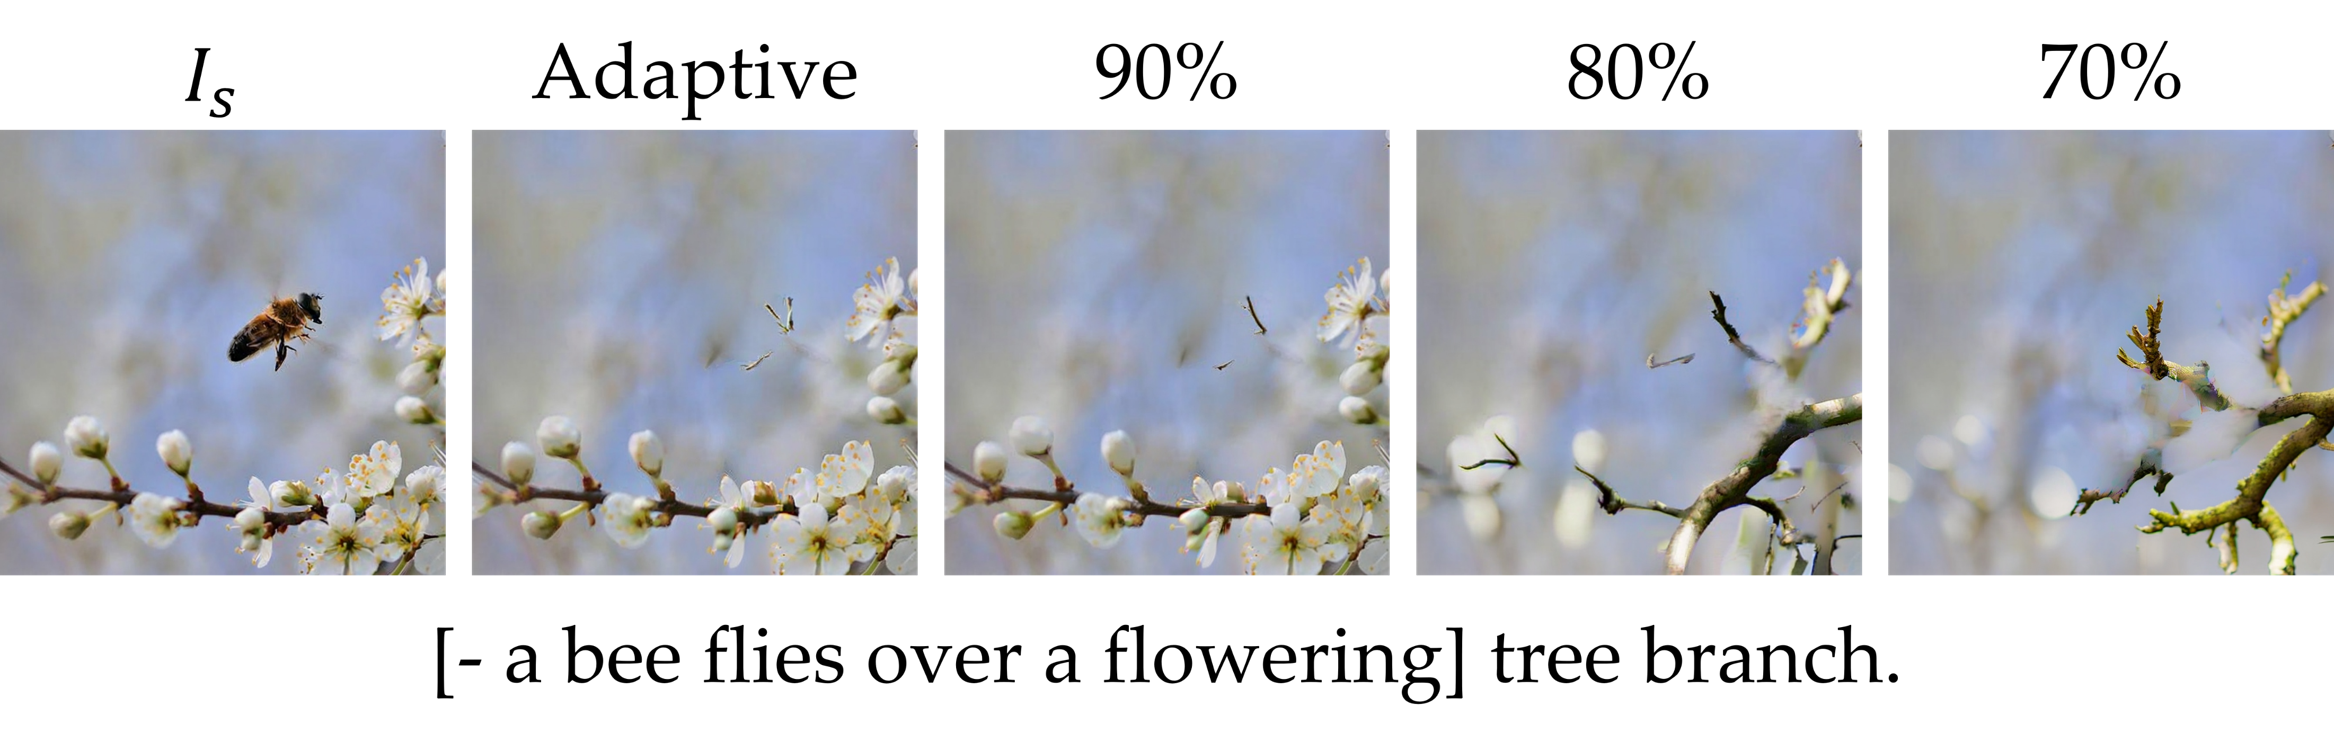
\includegraphics[width=\linewidth]{imgs/ablationDynamic.png}
    \caption{Effect of adaptive vs.\ fixed-percentile thresholding. $I_s$ denotes the source image. Adaptive thresholding produces fine-grained masks that preserve subtle structural details. While the 90\% fixed threshold yields reasonable results in this case, it still misses fine details that adaptive thresholding captures. The 70\% and 80\% thresholds generate overly coarse masks, causing the tree branch structure to be lost entirely.}
    \label{fig:ablationDynamic}
\end{figure}